\chapter{Introducción}\label{ch:intro}
\pagenumbering{arabic}
\section{Energía}\label{sec:energy}
La demanda global energética está aumentando en los últimos años principalmente debido al crecimiento demográfico y económico.
El continuo desarrollo de la sociedad moderna requiere que las fuentes de energía sean sostenibles
y respetuosas con el medio ambiente. Sin embargo, hoy en día más del 80\% de la energía mundial proviene
de combustibles fósiles~\cite{/content/publication/caf32f3b-en}, incluyendo carbón, petróleo y gas natural, que están limitados en reserva.
Además, las emisiones de CO$_2$ de este tipo de energía es la principal contribución al aumento del 
efecto invernadero y tiene un efecto importante en el cambio climático. Se
sabe que para nuestro entorno de vida el nivel asequible de aumento de la
temperatura media por encima de los niveles antes de la era industrial es de 2 \centigrade C, más allá del cual es irreversible y casi
se espera que ocurra un cambio climático catastrófico e incontrolable. Este aumento ya ha alcanzado los 0.78 \centigrade C~\cite{ip02000c}.
Por lo tanto, es urgente encontrar una manera de reducir la energía relacionada con
los combustibles fósiles. Un alivio a corto plazo sería el desarrollo de nuevas tecnologías para
reducir las emisiones de CO$_2$ de las plantas de energía fósil y mejorar el almacenamiento de CO$_2$ a gran escala,
mientras que una solución a largo plazo debería considerar las alternativas a los combustibles fósiles. Los candidatos con recursos suficientes para hacerse cargo del abastecimiento son la energía solar, la fisión y
la fusión nucleares~\cite{Freidberg:1186225}.\par
La energía solar es teóricamente amplia e inagotable, pero su intermitencia (luz solo en días sin nubes) y la baja densidad energética (se requiere una gran superficie) hacen difícil construir
una planta de energía solar para producir una cantidad significativa de energía base. La fisión nuclear es
una fuente de energía bien establecida y ha estado produciendo electricidad de carga base durante décadas.
Sin embargo, la eliminación de los residuos nucleares de larga y media vida junto al riesgo de accidente debido a la
reacción en cadena intrínseca de la fisión nuclear ha sido durante mucho tiempo una preocupación pública.\par
La fusión nuclear promete una solución limpia y segura para nuestras necesidades energéticas a largo plazo~\cite{Freidberg:1186225}. 
Primero, las reservas de combustible son abundantes. Para la reacción se necesitan deuterio y tritio, el deuterio puede ser 
extraído del agua de mar; el tritio no se produce de forma natural, pero puede ser obtenido a partir del isótopo de litio $^6$Li. 
Segundo, las reacciones de fusión nuclear no emiten gases de efecto invernadero o cualquier otro daño químico a la atmósfera. 
Tercero, la fusión nuclear es intrínsecamente segura. El combustible de fusión se introduce continuamente en el reactor a una velocidad que sostiene la reacción durante sólo unas pocas decenas
de segundos en cada instante. La reacción de fusión sólo puede ocurrir bajo una temperatura muy alta
y un campo de confinamiento suficientemente preciso y sin reacción en cadena. Cualquier manipulación incorrecta detendrá la reacción.\par
\section{Fusión nuclear}\label{sec:fusion}
Los protones y neutrones en el núcleo se mantienen unidos por la fuerza nuclear de corto alcance. La energía
requerida para desmontar un núcleo se llama energía de enlace. La figura~\ref{fig:nucleons} muestra que el promedio
de la energía de enlace varía entre elementos; tanto los núcleos más ligeros como los más pesados tienen un promedio bajo
y los núcleos de masa intermedia tienen la mayor energía de unión.
Esto muestra que la energía nuclear puede obtenerse tanto por la división de núcleos pesados (fisión) como 
fusionando los núcleos ligeros (fusión).\par
\begin{figure}
    \centering
    \def\svgwidth{10cm}
    \input{svg/bindingenergy.pdf_tex}
    \caption[Energía de enlace]{Energía de enlace promedio en función del número másico.}
    \label{fig:nucleons}
\end{figure}
Para lograr una reacción de fusión, dos núcleos necesitan ganar suficiente energía cinética como para superar
la repulsión de Coulomb y alcanzar el régimen de fuerza nuclear de corto alcance. La primera fusión 
se realizó experimentalmente bombardeando sobre un deuterio
objetivo ($^2$H o D) con un rayo de deuterio~\cite{Oliphant1934}, justo después del descubrimiento del deuterio (el isótopo de hidrógeno de masa dos~\cite{PhysRev.40.1}).
Fue durante estos experimentos que el tercer isótopo de hidrógeno, el tritio ($^3$H o T),
se descubrió. Después de este logro, el uso de la fusión nuclear como fuente de energía fue
considerado. Sin embargo, se reconoció que bombardear un objetivo con un chorro acelerado de partículas 
no es factible para la generación de energía, porque la energía utilizada para la aceleración de la partícula
es mucho mayor que la energía producida por la reacción de fusión nuclear y la mayoría de
las partículas aceleradas no daban en el objetivo.\par
\begin{figure}
    \centering
    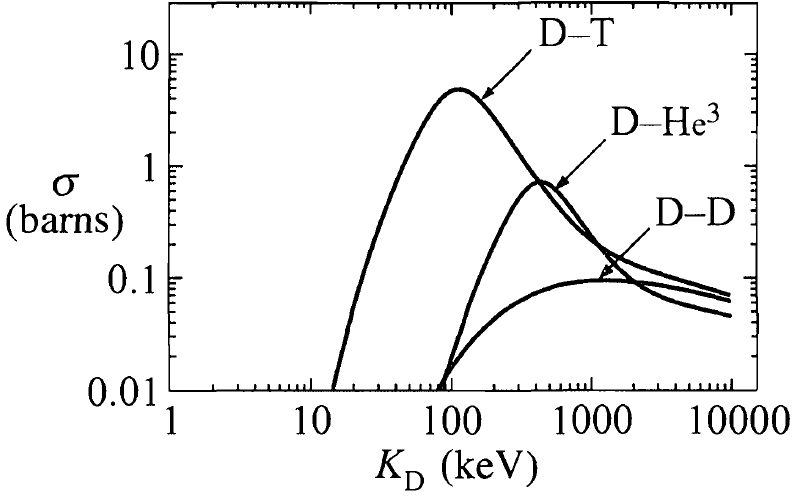
\includegraphics[scale=0.5]{img/fusion.png}
    \caption[Secciones eficaces en reacciones de fusión]{Secciones eficaces para las reacciones de fusión D-T, D-$^3$He y D-D en función de la energía cinética del deuterón $K_D$~\cite{Freidberg:1186225}.}
    \label{fig:fusion}
\end{figure}
Hoy en día se acepta generalmente que la forma más factible para la producción efectiva de energía 
con fusión nuclear es calentar los combustibles de fusión a alta temperatura, para que las partículas se acerquen
con un fuerte movimiento térmico y una reacción nuclear pueda tener lugar. A tan alto nivel de
temperatura, los combustibles de fusión están ionizados y en un estado llamado plasma. La figura~\ref{fig:fusion} muestra las
secciones transversales (probabilidad de que ocurra una reacción nuclear) de diferentes reacciones nucleares.
Podemos ver que la reacción más prometedora es entre el deuterio y el tritio produciendo el neutrón
y una partícula $\alpha$.
\begin{equation}\label{eq:deutreaction}
    D+T\rightarrow\ce{^{4}He}\;(3.5\;\mathrm{MeV})+n\;(14.1\;\mathrm{MeV})
\end{equation}
La energía producida es transportada como energía cinética por el neutrón y la partícula $\alpha$.\par
Uno de los objetivos fundamentales para obtener energía de fusión es mantener el alta temperatura, no con el calentamiento 
externo sino con la energía producida por la reacción nuclear en sí. Este
proceso se llama ignición. Para alcanzar la ignición, el criterio de Lawson~\cite{Lawson_1957} predice que 
debe cumplirse la siguiente condición:
\begin{equation}\label{eq:lawson}
    nT\tau_e\geq3\times10^{21}\:keVs/m^{3}
\end{equation}
donde n es la densidad del plasma, T es la temperatura y $\tau_e$ es el tiempo de confinamiento produciendo energía.
Este triple producto sugiere que para generar energía de forma efectiva a partir de la fusión nuclear, el plasma
necesita estar confinado a muy alta temperatura por un tiempo suficientemente largo con alta densidad.
Hay principalmente dos formas de conseguir energía de fusión controlada: el confinamiento magnético 
y el confinamiento inercial. Este trabajo se centra en la primera de ellas.\par
\section{Confinamiento magnético}\label{sec:confinement}
El confinamiento magnético de plasmas de alta densidad y temperatura es estudiado
desde hace varias décadas con la finalidad de construir un reactor de fusión que sea capaz
de producir energía. Para ello, es necesario conseguir la ignición del plasma. Esta se alcanza
cuando se cumple el criterio de Lawson~\eqref{eq:lawson}.
El tiempo de confinamiento de las primeras máquinas era de unos pocos milisegundos, dado
que el campo magnético confinante únicamente tenía componente toroidal. Se consiguieron
plasmas con un tiempo de confinamiento treinta veces superior cuando los campos magnéticos
tenían cierta helicidad. Para definir esta propiedad en \textit{stellarators}, se utiliza la transformada
rotacional que es el número de giros poloidales por cada giro toroidal. Normalmente este
valor varía a lo largo del radio, por ello se habla de perfil de la transformada rotacional. En
algunos puntos radiales el valor de la transformada rotacional puede ser racional, dando lugar
a superficies magnéticas resonantes. Esto sumado al hecho de que el plasma es un medio con
cierta resistividad, puede dar lugar al nacimiento de islas magnéticas que son superficies de
flujo que se forman dentro de la columna de plasma aisladas del resto de superficies magnéticas.
Son numerosos los estudios analíticos, numéricos y experimentales que se han realizado
para determinar si las islas magnéticas aumentan el transporte radial y con ello se reduce el
tiempo de confinamiento, pero la comunidad científica no ha llegado ningún acuerdo.\par
Otro fenómeno que provoca elevados niveles de transporte radial de partículas y energía
y en consecuencia una reducción del tiempo de confinamiento es la turbulencia. Para llevar a
cabo estudios que permitan reducir la turbulencia en el plasma, es necesario caracterizarla
previamente, para ello se emplean distintas magnitudes. Una de las más utilizadas es la longitud
de correlación radial ($L_r$). Se trata de una medida estadística de la turbulencia cuyo
valor es proporcional al tamaño de las estructuras turbulentas.
Son varios los diagnósticos que pueden medir $L_r$: sondas de Langmuir, \textit{Beam Emission Spectroscopy},
\textit{Heavy Ion Beam probe}, reflectometría, etc.
\subsection{Plasma}\label{subsec:plasma}
Un plasma es un gas ionizado, en el que los electrones son separados de los iones. La separación
de partículas cargadas positiva y negativamente da lugar a campos eléctricos. Los electrones son más
móviles que los iones en un plasma debido a la pequeña masa del electrón. Por lo tanto, la pequeña separación de la carga
puede dar lugar a la oscilación electrostática de los electrones alrededor de los iones de fondo.
La frecuencia de esta oscilación se llama frecuencia de plasma, $\omega_p^2=\left(\frac{n_ee^2}{\varepsilon_0m_e}\right)^{\frac{1}{2}}$ donde $n_e$  es la densidad electrónica del plasma, e es la carga del electrón, $\varepsilon_0$ es la constante dieléctrica del vacío y $m_e$ es la masa del electrón.
El rápido movimiento de los electrones consigue apantallar el desequilibrio de la carga, dotando de carga neutra a nuestro plasma (en mayor parte). 
La escala de longitud sobre la cual los electrones apantallan el desequilibrio de la carga es la longitud de Debye, $\lambda_D=\left(\frac{\varepsilon_0k_BT_e}{e^2n_e}\right)^{\frac{1}{2}}$
donde $T_e$ es la temperatura del electrón.\par
\begin{figure}
    \centering
    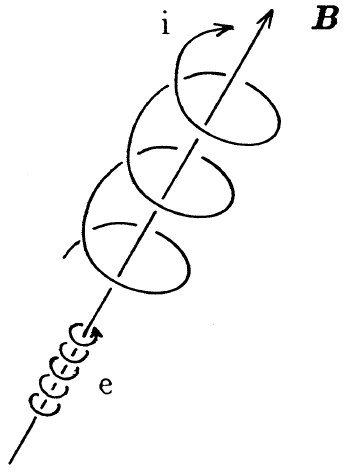
\includegraphics[scale=0.5]{img/larmor.png}
    \caption[Movimiento del electrón y el ion en un campo magnético]{Movimiento del electrón y el ion en un campo magnético~\cite{Miyamoto2011}.}
    \label{fig:larmor}
\end{figure}
Cuando una partícula cargada se mueve con velocidad \textbf{v} a través de un campo eléctrico \textbf{E} y magnético 
\textbf{B}, la fuerza electromagnética ejercida sobre la partícula cargada es la fuerza de Lorentz. Despreciando 
la gravedad, la ecuación del movimiento está dada por:
\begin{equation}\label{eq:lorentz}
    m\frac{d\textbf{v}}{dt}=q(\textbf{E}+\textbf{v}\times \textbf{B})
\end{equation}
\par
En un campo magnético uniforme, la partícula cargada sigue un movimiento helicoidal alrededor de la
línea de campo de la figura~\ref{fig:larmor}. Este movimiento puede descomponerse en un movimiento lineal (centros de giro)
a lo largo de la línea de campo y un movimiento circular, el movimiento de Larmor, perpendicular a la línea de campo.
Considerando la ecuación de fuerza de Lorentz~\eqref{eq:lorentz}, obtenemos la frecuencia ciclotrón $\omega_c$ y 
el radio de Larmor $r_L$ del movimiento como:
\begin{equation}\label{eq:ciclotron}
    \omega_c=\frac{\lvert q\rvert B}{m}
\end{equation}
\begin{equation}\label{eq:radiolarmor}
    r_L\equiv\frac{v_\perp}{\omega_c}=\frac{mv_\perp}{\lvert q\rvert B}
\end{equation}
\par
En unos campos genéricos \textbf{E} y \textbf{B}, es decir, \textbf{E} y \textbf{B} pueden variar en el espacio y en el 
tiempo, los centros de giro del movimiento pueden tener deriva a través de los campos magnéticos. Basado en lo que origina 
la deriva, el posible centro de giro se puede descomponer como: $\textbf{E}\times\textbf{B}$, $\nabla B$, curvatura 
y deriva por polarización $V_g=V_E+V_{\nabla B}+V_\kappa+V_p$. Todas estas derivas surgen básicamente debidas al 
cambio o distorsión de las órbitas de Larmor durante el movimiento de giro. Un centro de giro fundamental 
es $\textbf{E}\times\textbf{B}$: $V_E=\frac{\textbf{E}\times\textbf{B}}{B^2}$. 
Esta es el fundamento para controlar las inestabilidades a pequeña escala en un plasma.
\begin{figure}
    \centering
    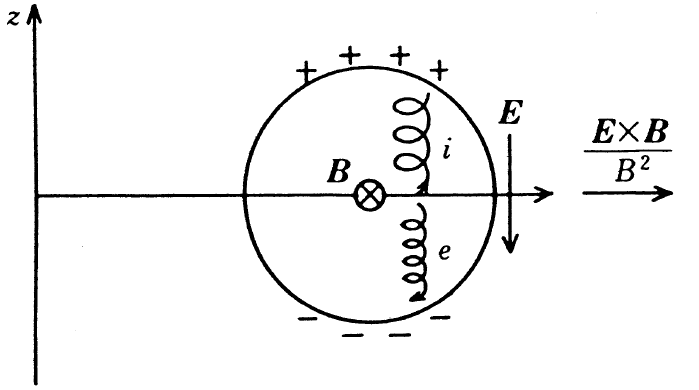
\includegraphics[scale=0.5]{img/drift.png}
    \caption[Deriva causada por un campo toroidal]{Deriva causada por un campo toroidal~\cite{Miyamoto2011}.}
    \label{fig:drift}
\end{figure}
\par
Las derivas de los centros de giro nos acercan a la comprensión del confinamiento del plasma. 
Debido a la alta movilidad de las partículas cargadas en el campo magnético, siempre hay un 
rápido \textit{end loss} en un dispositivo de líneas de campo abiertas, como en un cilindro recto o en 
<<espejos magnéticos>>. Para evitar este \textit{end loss}, la configuración principal para el 
confinamiento magnético es el toro. En un toro simple, podría ocurrir una deriva vertical de 
partículas (por ejemplo, debido a la deriva $\nabla B$) y causar la separación de las partículas 
cargadas. Esta separación da lugar a campos eléctricos. 
La fuerza producida por $\textbf{E}\times\textbf{B}$ moverá el plasma hacia afuera y degradará su confinamiento. 
Esta separación de carga puede ser compensada torciendo helicoidalmente las líneas 
de campo magnético alrededor del toro, es decir, el campo magnético total está formado por 
la combinación de un componente toroidal $B_\phi$ y un componente poloidal $B_\theta$. El número de 
tránsitos poloidales por cada tránsito toroidal de un campo en una superficie de flujo toroidal 
es la transformada rotacional $\iota/2\pi$.
\begin{equation}\label{eq:transrot}
    \frac{\iota}{2\pi}=\frac{d\psi}{d\Phi}
\end{equation}
donde $\psi$ es el flujo magnético poloidal, y $\Phi$ el flujo magnético toroidal. Más intuitivamente, si
las líneas de campo se cierran sobre sí mismas después de n tránsitos poloidales y m 
toroidales del toro, entonces $\iota=n/m$.\newpage
Hay básicamente tres maneras de retorcer el campo magnético, y por lo tanto crear una transformada rotacional~\cite{Helander_2012}:
\begin{enumerate}[(1)]
    \item llevando a deriva la corriente toroidal;
    \item alargando las superficies de flujo y haciendo que giren poloidalmente alrededor del toro;
    \item haciendo que el eje magnético no sea plano.
\end{enumerate}
\begin{figure}[H]
    \centering
        \minipage{0.32\textwidth}
            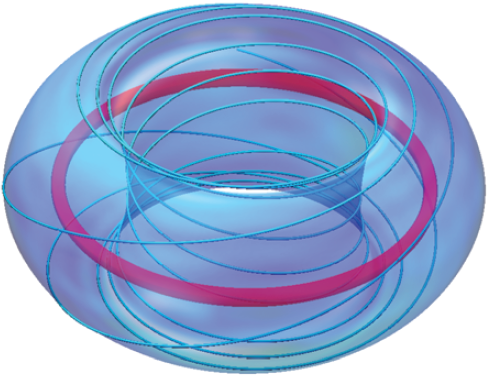
\includegraphics[width=\linewidth]{img/twist_1.png}
            \caption*{Tokamak}
        \endminipage\hfill
        \minipage{0.32\textwidth}
            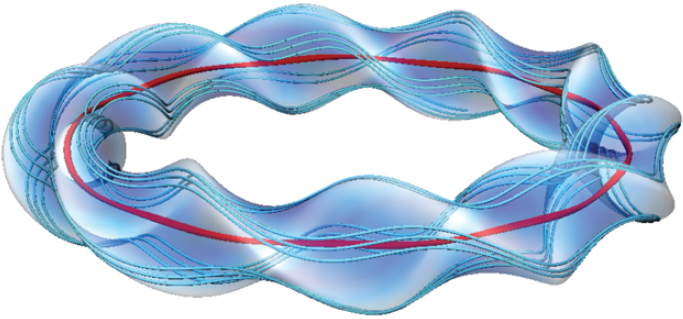
\includegraphics[width=\linewidth]{img/twist_2.png}
            \caption*{LHD \textit{stellarator}}
        \endminipage\hfill
        \minipage{0.32\textwidth}
            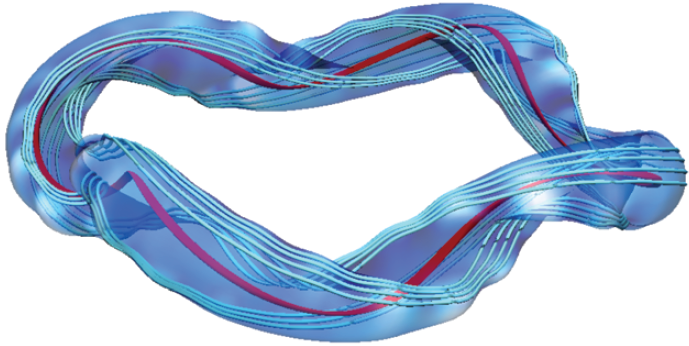
\includegraphics[width=\linewidth]{img/twist_3.png}
            \caption*{TJ-II \textit{stellarator}}
        \endminipage
    \caption[Superficies de flujo externo, líneas de campo y eje magnéticos para \textit{tokamak}, \textit{stellarator} LHD, y \textit{stellarator} TJ-II]{Superficies de flujo externo (azul transparente), líneas de campo magnético (azul claro) y eje magnético
    (rojo) para \textit{tokamak}, \textit{stellarator} LHD, y \textit{stellarator} TJ-II~\cite{doi:10.1063/1.4921255}.}
    \label{fig:twist}
\end{figure}
\par
La configuración magnética de los dispositivos de fusión toroidal se distingue principalmente
a través de la forma de generar la transformación rotacional. El \textit{tokamak}
usa el método (1). Algunos \textit{stellarators}, por ejemplo, el LHD, utilizan el método (2). Otros \textit{stellarators}, por 
ejemplo, TJ-II y W7-X utilizan tanto (2) como (3). Algunos diseños más avanzados, por ejemplo,
NCSX, utiliza los tres métodos. La figura~\ref{fig:twist} muestra las diferentes maneras de generar estas transformaciones.
La eficiencia del confinamiento del plasma por el campo magnético se mide por
el parámetro plasma beta, definido como la relación entre la presión del plasma y la presión magnética.
\begin{equation}\label{eq:beta}
    \beta=\frac{\langle p\rangle}{B^2/2\mu_0}
\end{equation}